% Séquence 1 : Les nombres entiers
\setseqtitle{Les nombres entiers}
\chapter{Les nombres entiers}

\section{Rang des chiffres}

\begin{definitionbox}
	\textbf{Chiffres et valeur}
	\begin{itemize}[label = \textbullet]
		\item 0, 1, 2, 3, 4, 5, 6, 7, 8, 9 sont les dix \textbf{chiffres} qui permettent d'écrire tous les nombres.
		\item Chaque chiffre a une \textbf{valeur} en fonction de sa position dans le nombre.
	\end{itemize}
\end{definitionbox}

On peut utiliser un tableau de numération pour visualiser le rang d'un chiffre.

\begin{center}
	\newcolumntype{C}{>{\centering\arraybackslash}p{1cm}}
	\begin{tabular}{|C|C|C|C|C|C|C|C|C|C|C|C|}
		\hline
		\multicolumn{3}{|c|}{\textbf{Classe des milliards}} & 
		\multicolumn{3}{|c|}{\textbf{Classe des millions}} & 
		\multicolumn{3}{|c|}{\textbf{Classe des milliers}} & 
		\multicolumn{3}{|c|}{\textbf{Classe des unités}} \\
		\hline
		\textbf{c} & \textbf{d} & \textbf{u} & 
		\textbf{c} & \textbf{d} & \textbf{u} & 
		\textbf{c} & \textbf{d} & \textbf{u} & 
		\textbf{c} & \textbf{d} & \textbf{u} \\
		\hline
		& & & & & & & & & & & \\
		\hline
	\end{tabular}
\end{center}

\textbf{Remarque :} Lorsqu'on écrit un nombre en chiffres, il faut laisser un espace entre les classes. Par exemple le nombre suivant 25204879603 s'écrit: \trous{2.5cm}.

\section{Décomposition décimale}

On peut donner la décomposition décimale de 3 584 :

\begin{examplebox}
	3 584 = (\trous{1.5cm} $\times$ \trous{2cm}) + (\trous{1.5cm} $\times$ \trous{2cm}) + (\trous{1.5cm} $\times$ \trous{2cm}) + \trous{1.5cm} $\times$ \trous{1cm}
\end{examplebox}



\textbf{Attention !} Pour le nombre 3 584, le chiffre des centaines est \trous{2cm} mais le nombre de centaines est \trous{3cm} (il y a \trous{2cm} centaines dans le nombre 3584).

En effet :
\trous{12cm}

\trous{12cm}

\section{Écriture en toutes lettres}

\begin{examplebox}
	\begin{itemize}[label = \textbullet]
		\item 1823 : Mille-huit-cent-vingt-trois (pas de << s >> à << cent >>, ni à << vingt >> car ils sont suivis d'autres chiffres !)
		\item 2087 : Deux-mille-quatre-vingt-sept (le mot << mille >> est invariable, et toujours pas de << s >> à << vingt >>...)
		\item 600 : Six-cents (ici on met bien un << s >> car il n'y a plus rien derrière !)
		\item 680 : Six-cent-quatre-vingts (pas de << s >> à << cent >>, mais un << s >> obligatoire à << vingt >> car le nombre se termine par 80).
	\end{itemize}
\end{examplebox}

Voici les règles correspondantes à ces exemples :

\begin{itemize}
	\item Le mot << mille >> est invariable ; les mots << million >> et << milliard >>, cependant, s'accordent et prennent donc un << \textbf{s} >> au pluriel.
	\item Les mots << cent >> et << vingt >> prennent un << \textbf{s} >> au pluriel uniquement lorsqu'ils sont à la fin du nombre.
	\item \textbf{Exemples :} 300 : \trous{3cm} \qquad 420 : \trous{4cm}
	\item Le mot << vingt >> ne s'utilise au pluriel (avec un << s >>) que si un nombre se finit par 80 (quatre-vingts).
	\item Les tirets sont mis entre chaque mot d'un nombre qui se présente sous forme composée. Avec des nombres entiers, il y aura donc des tirets partout !
	\item \textbf{Exemples :} 79 : \trous{4cm} \qquad 1031 : \trous{5cm}
\end{itemize}

\section{Demi-droite graduée}

\begin{definitionbox}
	\textbf{Demi-droite graduée}
	
	On appelle \textbf{demi-droite graduée} une demi-droite sur laquelle on fixe :
	\begin{itemize}[label = \textbullet]
		\item Un point appelé \textbf{origine de la demi-droite}
		\item \textbf{Un sens} représenté par une flèche
		\item \textbf{Une unité de longueur} que l'on reporte régulièrement à partir de l'origine.
	\end{itemize}
\end{definitionbox}

% Schéma de droite graduée avec TikZ
\begin{center}
	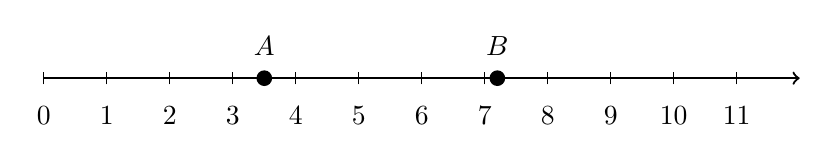
\begin{tikzpicture}[scale=0.8]
		% Droite graduée
		\draw[thick, ->] (0,0) -- (12,0);
		
		% Graduations
		\foreach \x in {0,1,...,11} {
			\draw (\x,-0.1) -- (\x,0.1);
			\node[below] at (\x,-0.3) {\x};
		}
		
		% Point A
		\node[circle,fill=black,inner sep=2pt] at (3.5,0) {};
		\node[above] at (3.5,0.2) {$A$};
		
		% Point B
		\node[circle,fill=black,inner sep=2pt] at (7.2,0) {};
		\node[above] at (7.2,0.2) {$B$};
	\end{tikzpicture}
\end{center}

\textbf{Exemple :} Sur cette demi-droite graduée, le point $A$ a pour abscisse \trous{1.5cm} et le point $B$ a pour abscisse \trous{1.5cm}.

\section{Comparaison de nombres entiers}

\begin{definitionbox}
	\textbf{Comparaison de nombres entiers}
	
	Pour comparer deux nombres entiers, on peut :
	\begin{itemize}
		\item Les placer sur une demi-droite graduée
		\item Comparer le nombre de chiffres
		\item Comparer chiffre par chiffre en partant de la gauche
	\end{itemize}
\end{definitionbox}

\begin{examplebox}
	Comparons 2 847 et 2 853 :
	\begin{itemize}
		\item Les deux nombres ont 4 chiffres
		\item On compare les milliers : 2 = 2
		\item On compare les centaines : 8 = 8
		\item On compare les dizaines : 4 < 5
		\item Donc 2 847 < 2 853
	\end{itemize}
\end{examplebox}

\textbf{Remarque :} Plus un nombre est à droite sur la demi-droite graduée, plus il est grand.

\section{Exercices d'application}

\begin{exercisebox}
\textbf{Exercice 1 :} Écris en toutes lettres les nombres suivants :
\begin{enumerate}
	\item 1 234
	\item 5 678
	\item 12 345
	\item 100 000
\end{enumerate}
\end{exercisebox}

\begin{exercisebox}
\textbf{Exercice 2 :} Place les points $A$, $B$, $C$ et $D$ d'abscisses respectives 2, 7, 4 et 9 sur une demi-droite graduée.
\end{exercisebox}

\begin{exercisebox}
\textbf{Exercice 3 :} Compare les nombres suivants en utilisant les symboles <, > ou = :
\begin{enumerate}
	\item 1 234 \trous{1cm} 1 243
	\item 5 678 \trous{1cm} 5 678
	\item 12 345 \trous{1cm} 12 354
\end{enumerate}
\end{exercisebox}

\section{Évaluation rapide (5 à 10 min)}

\begin{exercisebox}
\textbf{Mini-quiz :}
\begin{enumerate}
	\item Écris en toutes lettres : 8 765
	\item Quel est le chiffre des centaines dans 12 345 ?
	\item Place le point $E$ d'abscisse 6 sur une demi-droite graduée
\end{enumerate}
\end{exercisebox}

